\documentclass[8pt, landscape, fleqn]{scrartcl}
\setlength{\parindent}{0pt}
\usepackage[ngerman]{babel}
%\usepackage[applemac]{inputenc}
\usepackage[utf8]{inputenc}
\usepackage[dvips]{geometry}
\usepackage{latexsym}
\usepackage{multicol}
\usepackage{amsmath}
\usepackage{graphicx}
\usepackage{array}
\usepackage{booktabs}
\usepackage{amsmath}
\usepackage{mathtools}
\usepackage{ulem}
\usepackage{amsfonts}
\usepackage{dsfont}
\usepackage{charter} %%% Schreibart
%\renewcommand{\familydefault}{\sfdefault}



%%%%%%%%%%Paket für Chemische Formeln
\usepackage{chemformula} 
\usepackage[version=3]{mhchem}
%%%%%%%%%%%%%%%%% Farbe
\usepackage{color}

\pagestyle{plain}
\typearea{20}
\columnsep 30pt
\columnseprule .4pt
\setlength{\extrarowheight}{0.9em}

\renewcommand{\arraystretch}{0.8}

\makeatletter
\renewcommand{\section}{\@startsection{section}{1}{0mm}%
{-2\baselineskip}{0.8\baselineskip}%
{\hrule depth 0.2pt width\columnwidth\hrule depth1.5pt
width0.25\columnwidth\vspace*{1.2em}\Large\bfseries\rmfamily}}
\makeatother


\makeatletter
\renewcommand{\subsection}{\@startsection{subsection}{1}{0mm}%
{-2\baselineskip}{0.8\baselineskip}%
{\hrule depth 0.2pt width\columnwidth\hrule depth0.75pt
width0.25\columnwidth\vspace*{1.2em}\large\bfseries\rmfamily}}
\makeatother

\makeatletter
\renewcommand{\subsubsection}{\@startsection{subsubsection}{1}{0mm}%
{-2\baselineskip}{0.8\baselineskip}%
{\hrule depth 0.2pt width\columnwidth\vspace*{1.2em}\normalsize\bfseries\rmfamily}}
\makeatother

\newcommand{\Mx}[1]{\begin{bmatrix}#1\end{bmatrix}}
\begin{document}
\part*{\LARGE\textrm{Advanced Techniques Risk Analysis of Technical Systems $\hfill$ Xeno Meienberg}}
\begin{multicols*}{3}

\section{Introduction, Definitions \& Overview}

\textbf{Reliability}

\begin{itemize}
    \item ... is a characteristic of an item, expressed by the probability that the item performs its required function under given conditions \emph{during} a stated time interval, i.e. $(0,t]$
    \item Item = entity for investigation, i.e. component, assembly, equipment, subsystem, system 
    \item from a \textbf{qualitative} point of view, reliability is defined as the ability of an item to \textbf{remain functional}
    \item from a \textbf{quantitative} point of view, reliability is defined as the probability that \textbf{no operational interruptions} will occur during a stated time interval $R(t)$
\end{itemize}

\textbf{Availability}

\begin{itemize}
    \item Point Availability (PA) is a characteristic of an item expressed by the probability that the item performs its function \textbf{at an instant of time} $t$
    \item Qualitatively, it can be described as the dependebility 
    \item Average Availability (AA), is the expected time at which the item can perform its required function
    \item Availability is used to express Point Availability in a sloppy way or Average Availability
\end{itemize}

In comparison to Availability, the Reliability analysis includes the fact that no item is allowed to fail. This means, the function performed cannot be interrupted (redundant system however can be repaired). Availability incurs that failures can happen on the item level. \newline \newline

\textbf{Risk}

\begin{itemize}
    \item RISK = POTENTIAL DAMAGE x UNCERTAINTY
    \item Dictionary: RISK = probability of damage to a person or an object
    \item We define RISK as a function of an...
    \begin{itemize}
        \item Accident Scenario, $S$
        \item Probability, $p$
        \item Consequence, $x$
    \end{itemize}
    \item We can quantify RISK on the so-called ``Farmer's Curve'
\end{itemize}

\begin{center}
    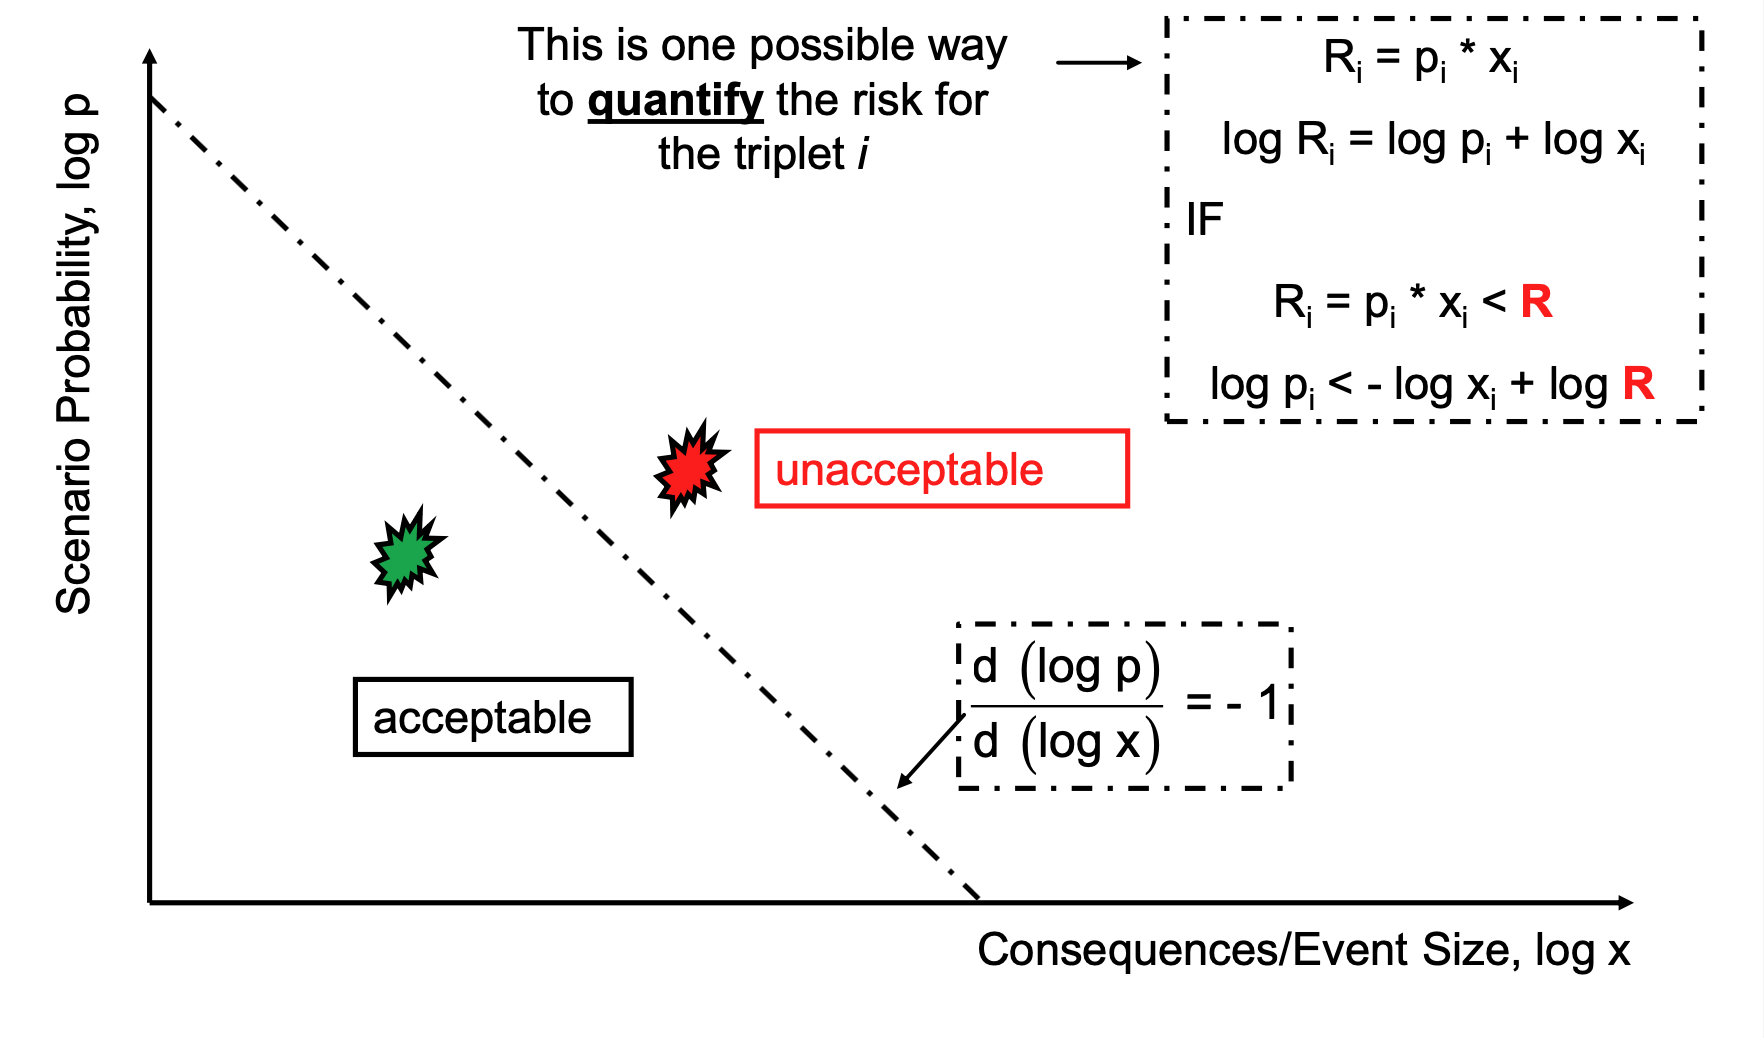
\includegraphics[width=8cm]{Images/Farmer_I.png}
    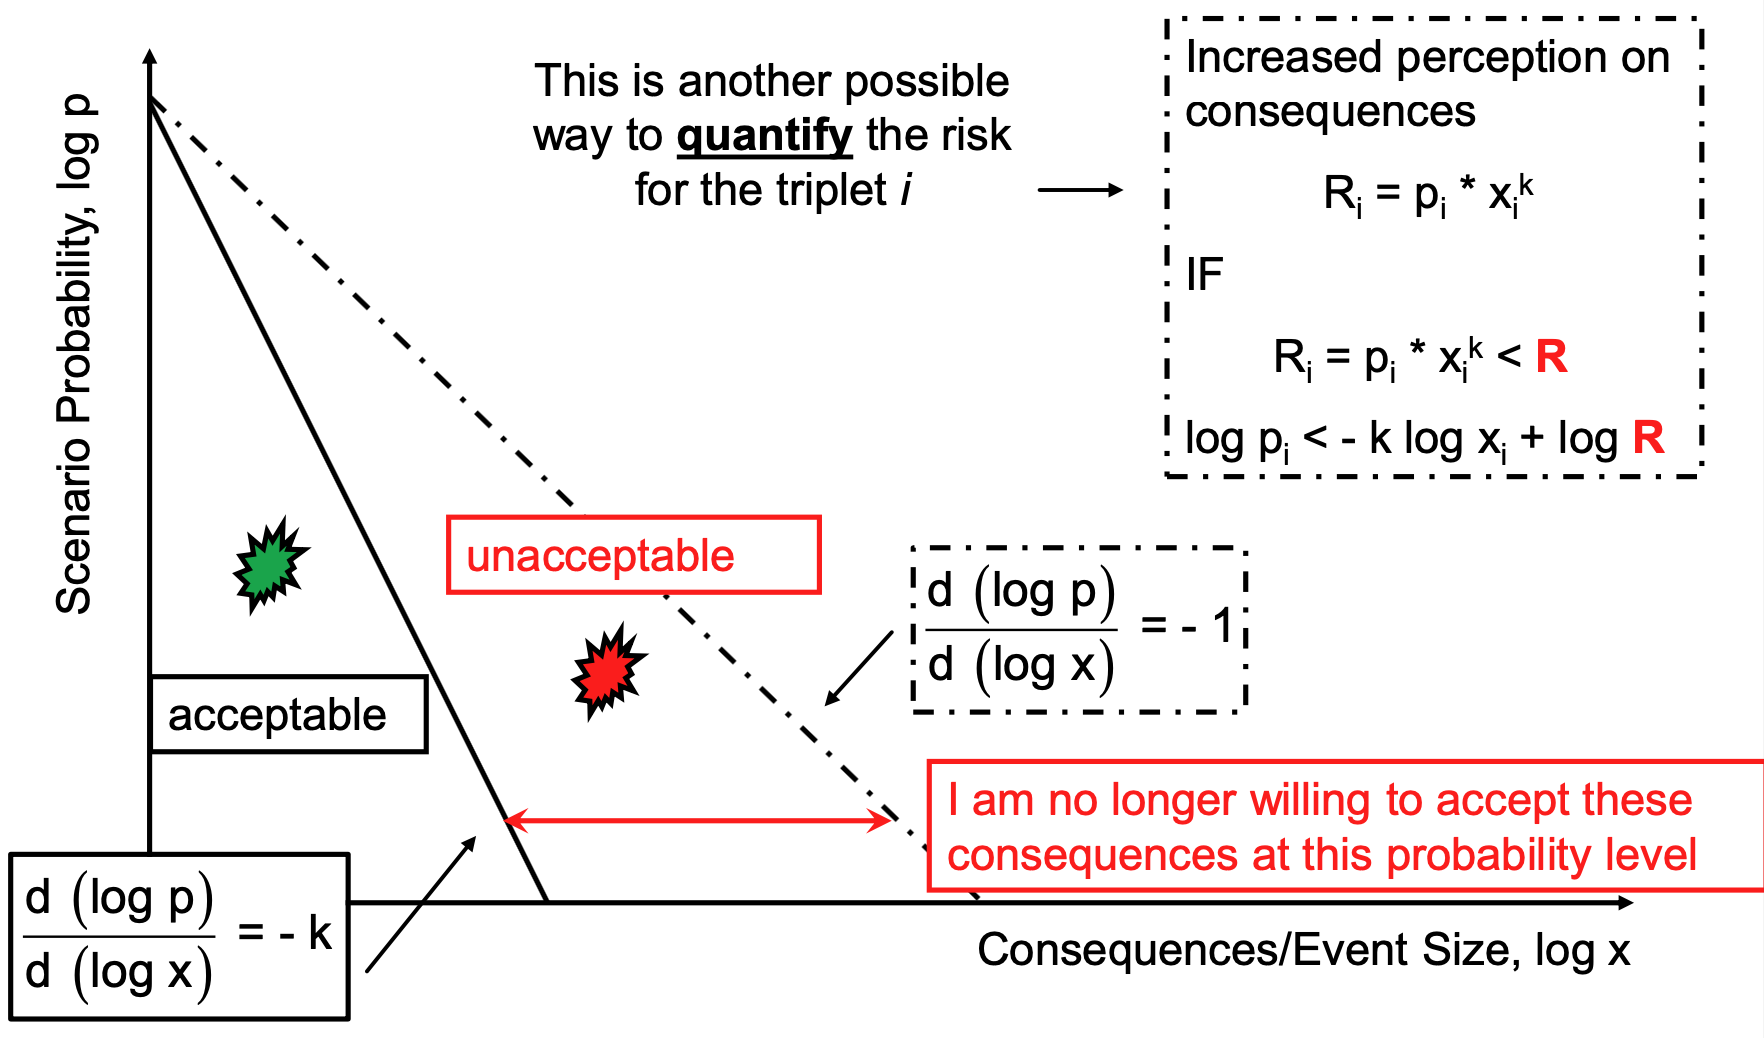
\includegraphics[width=8cm]{Images/Farmer_II.png}
\end{center}

The total Risk can be calculated as follows:

\begin{align}
    \text{Total Risk} = \sum p_i x_i^k, k\geq 1
\end{align}

It is entirely possible that the risk of different events can be dominated by either it's probability or its consequence. 

\begin{itemize}
    \item A large probability $p$ is \emph{prevented} of (minimisation based on high probability)
    \item A large consequence $x$ is \emph{mitigated, protected} (minimisation given its large impact)
\end{itemize}


\section{Probability Theory and Reliability Analysis}

Definitions:

\begin{itemize}
    \item Experiment $\epsilon$
    \item Sample space $\Omega$
    \item Event $E$
\end{itemize}

An event $E$ is a subset of the sample space $\Omega$ and the experiment $\varepsilon$ yields a set of possible outcoms ($= E$) of the experiment  \newline \newline \emph{Certain Events} follow \emph{Boolean Logic}, an event $E$ can occur or not occur, meaning an \emph{Indicator Variable} $X_E$ is 0 when $E$ does not occur and 1 if $E$ occurs \newline \newline
\emph{Uncertain Events} follow can either be true or false, with each a probability associated to it. Event $E$ in sample space $\Omega$ is triggered with a probability that the outcome has happened or not 

\subsubsection*{Classical Probability}

\begin{itemize}
    \item The experiment $\epsilon$ has $N$ possible, elementary, mutually exclusive and equally probable outcomes $A_1, A_2,..., A_N \in \Omega$
    \item The event $E = A_1 \cup A_2 \cup ... \cup A_M$,  $M\leq N$
    \item The probability of event $E$ is defined as $p(E) = M / N$
\end{itemize}

\subsubsection*{Kolmogorov Axioms}

\begin{enumerate}
    \item $0 \leq P(E) \leq 1$
    \item $P(\Omega) = 1$, $P(\emptyset) = 0$
    \item Mutually exclusive events: $P(\cup_i E_i) = \sum p(E_i)$
    \item Non-mutually exlusive events: \newline $P(A\cup B) = P_A + P_B - P(A \cap B)$
    \item Conditional probability: $P(A|B) = P(A\cap B) / P(B)$
    \item Theorem of total probability: Given an event $A$ in $\Omega$ where the space is consisting of exclusive and exhaustive events $\cup_j E_j = \Omega$: $P(A) = \Sigma_i(P(A | E_i)P(E_i))$
\end{enumerate}

\subsubsection*{Random Variables}

\begin{itemize}
    \item \textbf{CDF}: Is a non-decreasing function and returns the probabilty (state) from random variable $X$ from $0$ to a given point $A$: $F_X(X = A) = P(0 < X \leq A)$ 
    \item \textbf{pdf}: Probability of per unit $x$ (continuous)
    \item \textbf{pmf}: Histogram, it assignes the probability to discrete values $x$
\end{itemize}

\subsubsection*{Summary}

\begin{itemize}
    \item Distribution Percentile $x_\alpha$:
    \begin{itemize}
        \item $F_X(x_\alpha) = \alpha / 100 = \int_{-\infty}^{x_\alpha} f_X(x)dx$
    \end{itemize}
    \item Median:
    \begin{itemize}
        \item $F_X(x_50) = 0.5$
    \end{itemize}
    \item Mean:
    \begin{itemize}
        \item $\mu_X = E[X] = <X> = \sum_i x_i p_i$ (discrete)
        \item $= \int_{-\infty}^{\infty} x f_X(x) dx$ (continuous)
    \end{itemize}
    \item Variance:
    \begin{itemize}
        \item $\sigma_X^2 = \sum(x_i - \mu_X)^2 p_i$ (discrete)
        \item $ = \int_{-\infty}^\infty (x-\mu_X)^2 f_X(x) dx$ (continuous)
    \end{itemize}
\end{itemize}

\subsubsection*{Hazard Function (Failure Rate)}

 For risk and reliability analyses, we can use models whereas the time to failure of a component T can be expressed through a CDF $F_T(t)$ and a pdf $f_T(t)$. The complementary, cumulative function is 
 
 \begin{equation}
    R(t) = 1-F_T(t) = P(T\geq t)
 \end{equation}   

 which is decribed as the \textbf{Reliability or Survival Function} of the component T at time t and gives the probability of it surviving up to time t without failures. \newline 

 In order to monitor the failure evolution, given the component has survived up to time $t$ in a time interval $dt$, one can define a so called \textbf{Hazard Function or Failure Rate} $h_T(t)$. 

 \begin{align}
     h_T(t) dt = P(t< T \leq t + dt | T>t) = \\
     = \frac{P(t<T \leq t+t+dt)}{P(T>t)} = \frac{f_T(t)dt}{R(t)}
 \end{align}

 The hazard function is depending on time, and is often discribed through the bathtub curve. The failure rate at the beginning is higher (infant mortality, burn in) and decreses after a certain time. The failure rate becomes constant $\lambda$ and increases at the end through ageing. 

 \begin{center}
     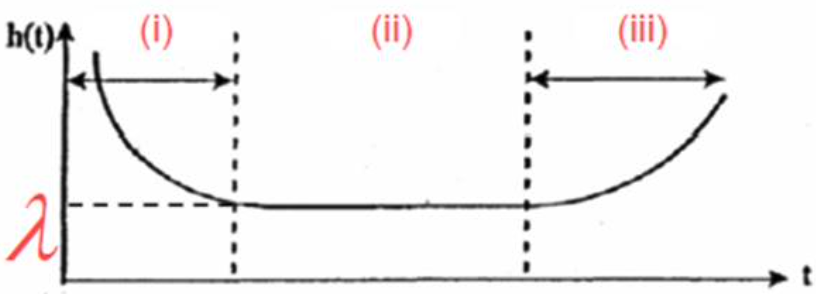
\includegraphics[width=6cm]{Images/Hazard_Function.png}
 \end{center}

 Through the definition of $R(t)$ and integrating the hazard function, we receive:

 \begin{align}
     F_T(t) = 1-e^{-\int_0^t h_T(\tilde{t}) d\tilde{t}} \\
     R(t) = e^{-\int_0^t h_T(\tilde{t}) d\tilde{t}}
 \end{align}

 If our hazard function is in its constant phase (constant hazard rate), the failure evolution follows the \textbf{Exponential Distribution}:

 \begin{align}
    h_T(t) \lambda, t>0 \\
     F_T(t) = P(T \leq t) = 1-e^{-\lambda t} \\
     R(t) = \begin{dcases}
         f_T(t) = \lambda e^{-\lambda t} & t \geq 0 \\
        0 & t < 0
     \end{dcases}
 \end{align}

 \begin{center}
     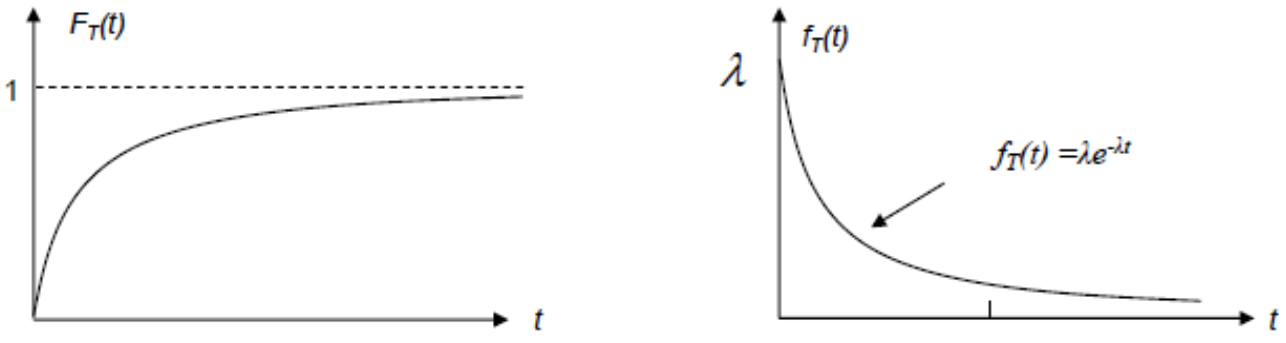
\includegraphics[width = 8cm]{Images/Exponential_Distribution.png}
 \end{center}

 The mean time to failure (MTTF) can be found through the expectation value

 \begin{align}
     E[T] = \frac{1}{\lambda} = MTTF \\
     Var[T] = \frac{1}{\lambda^2}
 \end{align}

 The failure process is memoryless. Given a component has survived at least until time $t_1$, the probability of it failing between time $t_1$ and $t_2$ is only depending on the time inbetween and not prior to time $t_1$

 \begin{align}
     P(t_1 < T < t_2) = \frac{P(t_1 < T < t_2)}{P(T > t_1)} = \frac{F_T(t_2)-F_T(t_1)}{1-F_T(t_1)} = \\
     \frac{e^{-\lambda t_1}-e^{-\lambda t_2}}{e^{-\lambda t_1}} = 1-e^{-\lambda(t_2-t_1)}
 \end{align}

The influence of an ageing process of the components failure rate shows that is not constant through time and hence can be described through the \textbf{Weibull distribution}. 

\subsubsection*{Boolean Logic - Fault Tree Analysis}

Fault trees = set of Boolean algebraic equations (one for each gate) $\rightarrow$ structure (switching) function $\Phi$

\begin{equation}
    X_T = \Phi(X_1,X_2,X_3,...,X_N)
\end{equation}

The top event is connected by an OR-gate, hence if one of each events is true, then the top event will be true. Here some further rules:

\begin{itemize}
    \item Negation: Given event $E$, given by the indicator variable $X_E$, its negation is described by $\overline{X_E} = 1-X_E$
    \item Intersection: The event $A \cap B$ is true, if both $A$ and $B$ are simultaneously true: \begin{equation} X_{A\cap B} = X_A X_B \end{equation} ($X_{A\cap B} = 0$ for mutually exclusive events)
    \item Union: The event $A \cup B$ is true, if either $A$ or $B$ are true and false if both are false: \begin{align} X_{A \cup B} = 1-(1-X_A)(1-X_B)\\= 1- \Pi(1-X_j) = \amalg X_j \\ = X_A + X_B - X_A X_B \end{align}
    \item Probability of event $E$ with expected value Operator $E(\cdot)$: $p(E) = E(X_E)$ \begin{equation}
        p(E) = p(X_E = 1)\cdot 1 + p(X_E = 0) \cdot 0 = E(X_E)
    \end{equation} 
    \item Multiple, non-mutually exclusive events: \begin{equation}
        X_\cap = \Pi X_i
    \end{equation}
    \item Probability of event $E_\cap$ for the intersection of n events: \begin{equation}
        P(E_\cap ) = E[X_\cap] = \Pi P(E_j) (\text{if events are independant})
    \end{equation}
    \item Union of event $E_\cup$ for the union of n events: \begin{align}
        X_\cup = 1 - \Pi(1-X_j) = X_A + X_B + X_C \\ - X_A X_B - X_A X_C - X_B X_C - X_A X_B X_C \end{align}
    \item Probability of even $E_\cup$ for the union of n events: \begin{align}
        P(E_\cup) = E[X_\cup] = \sum P(E_j) - \\ \sum \sum P(E_j \cap E_i ) + (-1)^{n+1}P(\cap E_j)
    \end{align}
\end{itemize}

\subsubsection*{Structure Function and Minimal Cut Sets}

\begin{itemize}
    \item Cut Set: Is a logical combination of primary event (\textbf{combination of component failures}) which render true the top event (\textbf{system failure})
    \item Minimal Cut Sets: Cut set that does not have another cut set as a subset. This means repairing one element of the set repairs the entire system. Therefore, removing one element of a MCS makes it no longer a cut set.
\end{itemize}

Any fault tree $\Phi(X)$ can be equivalently written as an OR-gate in the first level below the top event combining the minimal cut sets, each in return represented by
an AND-gate intersecting all elements comprising the given minimal cut set

\begin{align}
    \Phi(X) = 1- (1-M_1)(1-M_2)(1-M_3)...\\ ...(1-M_{mcs}) = \amalg^{mcs}_j M_j \\ P(\Phi(X)=1) = E[\sum M_j - \sum \sum M_i M_j+ ... \\ ... + (-1)^{mcs+1}\Pi M_j \\ = \sum P(M_j) - \sum \sum P(M_i M_j) + ... \\ ...+ (-1)^{mcs+1}P\left(\Pi M_j \right)
\end{align}

\begin{itemize}
    \item First event approximation: $\sum P(M_j)$
    \item Second event approximation: \\ $\sum P(M_j)-\sum_i^{mcs-1} \sum_j^{mcs} P(M_i M_j)$
\end{itemize}

Important fact: Idemponent law follows for Boolean values - $X * X = X$ 

\begin{align}
    P(M_1 M_2) = P(M_1 \cap M_2) = E[M_1 \cap M_2] = \\ E[X_1 X_2 \cap X_2 X_3 X_4] = E[X_1 X_2 X_2 X_3 X_4] \\ = E[X_1 X_2 X_3 X_4]
\end{align}

if both events M are independent, then

\begin{equation}
    P(M_1 M_2) = P(X_1)P(X_2)P(X_3)P(X_4) = p_k(T_m)^4
\end{equation}

The occurence probability of $X_2$ will only be appearing once in the calculation of the intersection of $M_1$ and $M_2$ and hence the Unreliability (Failure Rate) calculations become more exact through subtraction of the intersection (second event approximation) and will be bounded by both approximations:

\begin{equation}
    \sum P(M_j) - \sum \sum P{M_i M_j} < U_{mcs}(T_m) < \sum P(M_j)
\end{equation}

\subsubsection*{Reliability Analysis}

\textbf{Series System} 

\begin{itemize}
    \item All components must function in order of a functioning system 
    \begin{equation}
        R(t) = \Pi R_i(t) \end{equation}
    \item For $N$ exponential components:
    \begin{align}
        R(t) = e^{-\lambda t} \\
        \lambda = \sum \lambda_i (\text{System Failure Rate})\\
        E[T] = 1 / \lambda (\text{MTTF})
    \end{align}

\end{itemize}

\textbf{Parallel System}

\begin{itemize}
    \item All components must fail in order the system to fail
    \begin{equation}
        R(t) = 1 - \Pi \left[1- R_i(t)\right]
    \end{equation}
    \item For $N$ exponential components:
    \begin{align}
        R(t) = 1- \Pi \left[1 - e^{\lambda_i t}\right] \\
        MTTF = \sum 1/\lambda_i \sum \sum 1/(\lambda_i +\lambda_j) + ... \\
        ...+\sum \sum \sum 1/(\lambda_i +\lambda_j +\lambda_k) + ... \\ 
        ...+ (-1)^{N-1} 1/\sum\lambda_i
    \end{align}
    \item Example with two exponential units of failure rates $\lambda_1$ and $\lambda_2$:
    \begin{equation}
        MTTF = \frac{1}{\lambda_1} + \frac{1}{\lambda_2} - \frac{1}{[\lambda_1 + \lambda_2]}
    \end{equation}
    \item For N identical elements, compare series and parallel:
    \begin{align}
        \text{parallel}:~ MTTF = \sum_n^N \frac{1}{n\lambda} \\
        \text{series}: ~ MTTF = \frac{1}{N\lambda} \\ 
        MTTF_{parallel} < MTTF_{series}
    \end{align}
\end{itemize}


\subsection*{Markov Processes: Basic Elements}

\textbf{System}

\begin{itemize}
    \item The system can occupy a finite/countable number of states N
    \item The states are mutually exclusive, i.e. the system is in one state at each time 
    \item The states are exhaustive, i.e. the system must be in one state at all times 
\end{itemize}

\textbf{Transitions} between States occur \textbf{stochastically}, i.e. randomly in time \\ \\
\textbf{Mathematical Representation}

\begin{itemize}
    \item The random process of the state transition can be described by an integer random variable, e.g. $X(t) = 5$, the system occupies state $5$ at time $t$
    \item The stochastic process can be observed at discrete times, and we assume that time intervals between states is such small that only one transition occurs between two states
\end{itemize}

\textbf{The conceptual Model: Discrete States}

\begin{itemize}
    \item The state transition will be described by an integer random variable $X(n)$ is the system state at time $t_n$, $X(3) = 5$ means that the system occupies state $5$ at time $t_3$
    \item The objective is: Compute the probability that the system is in a given state at given time $t$, for all possible states and times
\end{itemize}

\begin{itemize}
    \item \textbf{In general stochastic processes:} The probability of a future state depends on its entire life history
    \item \textbf{In Markov processes:} The probability of a future state only depends on the present state. The process has no memory 
    \item The transition probability that the system in state $i$ at time $t_m$ moves to state $j$ at time $t_n$ \begin{align}
        p_{ij}(m,n) = P\left[X(n) = j | X(m) = i\right], n> m \geq 0 \\
        i = 0,1,2,...,N, j= 0,1,2,...,N
    \end{align}
\end{itemize}

\textbf{Properties of Transition Probabilities}

\begin{itemize}
    \item Transition probabilities are greater or equal to $0$
    \item Transitions must sum up to $1$
    \item $p_{ij}(m,n) = p[X(n)=j,X(m)=i] \\ = \sum_k p_{ik}(m,r)p_{kj}(r,n), \\ i=0,1,2,...,N, j=0,1,2,...,N$
\end{itemize}

\textbf{Stationary Transition Probabilities}

\begin{itemize}
    \item If the transition probability $p_{ij}(m,n)$ depends on the time interval ($t_n-t_m$) and not on the individual times $t_m$ and $t_n$, then
    \begin{itemize}
        \item The transition probabilities are stationary 
        \item The Markov Process is homogeneous in time 
    \end{itemize} \begin{equation}
        p_{ij}(m,n) = p_{ij}(k), k\geq 0, i,j=0,1,2,...,N
    \end{equation}
    \item We only need to know the \textbf{stationary one-step transition probabilities} $p_{ij}(1) = p_{ij}$
\end{itemize}

\textbf{The Transition Probability Matrix}:

\begin{equation}
    \uuline{A}_{ij} = \begin{pmatrix}
        p_{00} & p_{01} & ... & p_{0N} \\
        p_{10} & p_{11} & ... & p_{1N} \\
        \dots   & \dots & \dots & \dots \\
        p_{N0} & p_{N1} & ... & p_{NN}
    \end{pmatrix}
\end{equation}

\begin{itemize}
    \item $dim(A) = (N+1) x (N+1)$
    \item $0 \leq p_{ij} \leq 1, \forall i, j \in \{0,1,...,N\}$
    \item $\sum_j p_{ij} = 1$, hence only $(N+1)xN$ elements must be known 
    \item $\uuline{A}$ is a stochastic Matrix 
\end{itemize}


\textbf{Unconditional State Probabilities}:

\begin{align}
    \underline{P}(n) = \left[ P_0(n), P_1(n), ..., P_j(n),...,P_N(n)\right] = \\ \text{probabilities of being in state 0,1,...,N at time step n} \\
    \underline{P}(0) = \underline{C} = \left[C_0, C_1, ..., C_j,..., C_N\right] = \\ \text{initial vector at time step n=0}
\end{align}

At the first time step $n=1$:

\begin{align}
    P_j(1) = P[X(1) = j] \\ = \sum_{i=0}^N P\left[X(1) = j | X(0) = i\right] \cdot P\left[ X(0)=i\right] \\ = \sum_{i=0}^N p_{ij} C_i, \text{with } j = 0,1,2,...,N
\end{align}

The fundamental equation follows:

\begin{align}
    \underline{P}(n) = \underline{P}(0) \cdot \uuline{A}^n = \underline{C} \cdot \uuline{A}^n \\
    \uuline{A}^n = \begin{pmatrix}
        p_{00}(n) & p_{01}(n) & ... & p_{0N}(n) \\
        p_{10}(n) & p_{11}(n) & ... & p_{1N}(n) \\
        \dots   & \dots & \dots & \dots \\
        p_{N0}(n) & p_{N1}(n) & ... & p_{NN}(n)
    \end{pmatrix}
\end{align}

\begin{equation}
    p_{ij}(n) = P[X(n) = j | X(0) = i]
\end{equation}

The probability of arriving in state j after n steps given the initial state was i \newline \newline

\textbf{General Solution of the Fundamental Equation}

\begin{enumerate}
    \item Solve the eigenvalue ($\omega$) problem: $\underline{V}\cdot \uuline{A} = \omega \cdot \underline{V}$
    \item With the eigenvectors: $\underline{V_j} \cdot \uuline{A} = \omega_j \cdot \underline{V_j}$ 
    \item $\underline{P}(n) = \sum_{j=0}^N \alpha_j \cdot \underline{V_j}$ and $\underline{C} = \sum_{j=0}^N c_j \cdot \underline{V_j}$ are linear combinations of the eigenvectors
    \item The coefficients can be found through the adjoint eigenvalue problem
    \item The general solution yields: $\underline{P}(n) = \sum_{j=0}^{N} c_j\cdot \omega_j^n \cdot \underline{V_j} $
    \item The availability at time $k$: $A(k) = \sum_{j \in \text{success states}} P_j(k)$
\end{enumerate}

\textbf{Steady State Probabilities:}

\begin{enumerate}
    \item Solve $\underline{\Pi} = \underline{\Pi} \cdot \uuline{A}$ with $\sum_{j=0}^{N} \Pi_j = 1$ (2 equations)
\end{enumerate}

\textbf{First-passage Probabilities}

\begin{itemize}
    \item Probability that the system arrives \textbf{for the first time} in state j \textbf{after n steps}, given that it was in state i at the initial time 0 
    \begin{align*}
        f_{ij}(n) = P\left[X(n) = j \text{ for the first time} | X(0) = i\right] \\
            f_{ij}(n) = P\left[X(n) = j, X(m) \neq j, 0 < m < n | X(0) = i \right] \end{align*}
    \item Notice that $f_{ij}(n) \neq p_{ij}(n) = $ probability that the system reaches state $j$ \textbf{after $n$ steps} starting from state i, but \textbf{not necessarily for the first time}
\end{itemize}

\textbf{General Formula for the first-passage probability}

\begin{align}
    f_{ij}(k) = \underbrace{p_{ij}(k)}_{(I)}-\underbrace{\sum_{l=1}^{k-1} f_{ij}(k-l)p_{jj}(l)}_{(II)} \\ R(k) = 1- \sum_{l=1}^k \sum_{j \in \text{ failed states}} f_{ij}(l)
\end{align}

The probability of passing the state $j$ from $i$ is the transition probability at time step $k$, given it was in $i$ at $0$ $(I)$ whereas $(II)$ is the probability of staying in j as it reached the state prior to time step $k$ \\ \\ The reliability is defined as the probability at time $k$ where the system has not yet failed, hence we subtract all first passage probabilities of all failed states up to time $k$ \newline \newline \textbf{Recurrent, Transient and Absorbing States}


\begin{itemize}
    \item Recurrent: The system at state $i$ will surely return to $i$ \textbf{sooner or later}:
    \begin{equation}
        \Pi_i \neq 0
    \end{equation}
    \item Transient: The system at state $i$ has a \textbf{finite probability} of \textbf{never} returning to it:
    \begin{equation}
        \Pi_i = 0
    \end{equation}
    \item Absorbing: The state $i$ is absorbing if the system cannot leave it once it enters:
    \begin{equation}
        p_ii = 1
    \end{equation}
\end{itemize}

\newpage

\textbf{Average Occupation Time of a State}

\begin{itemize}
    \item The average occupation time of a stat i for $l_i$ steps = Average number of steps before the systems exits the state $i$:
    \begin{align}
        l_i [\text{steps}]= \frac{1}{P(\text{System exits state i})} \\ = \frac{1}{1-P(\text{System remains in i})} = \frac{1}{1-p_{ii}}
    \end{align}
\end{itemize}

\subsection*{Continuous-time Discrete-state Markov Processes}

What are they useful for?

\begin{itemize}
    \item Model the evolution of one component or system as a structure of components
    \item To find the probability that the system will be functioning at time $t^*$
\end{itemize}

\textbf{The transition probability matrix}

\begin{equation}
    p_{ij}(dt) = \alpha_{ij} \cdot dt + \underbrace{\theta(dt)}_{O(dt)},~\lim_{dt \rightarrow 0} \frac{\theta(dt)}{dt} = 0
\end{equation}

In analogy with the discrete-time formulation:

\begin{equation}
    \uuline{A} = \begin{pmatrix}
        1-dt\cdot \sum_{j=1}^{N} \alpha_{0j} & \alpha_{01} \cdot dt & ... & \alpha_{0N} \cdot dt \\
        \alpha_{10}\cdot dt & 1-dt\cdot \sum_{j=0, \neq 1}^{N} \alpha_{1j} & ... & \alpha_{1N} \cdot dt \\
        ... & ... & ...& ...
    \end{pmatrix}
\end{equation}

\begin{align}
    \underline{P}(t+dt) = \underline{P}(t)\cdot \uuline{A} \\
    \frac{d\underline{P}}{dt} = \underline{P}(t) \cdot \uuline{A}^* \\
    \underline{P}(0) = \underline{C}
\end{align}

\begin{equation}
    \uuline{A}^* = \begin{pmatrix}
        -\sum_{j=1}^N \alpha_{0j} = \alpha_{00} & \alpha_{01} & ... &  \alpha_{0N} \\
        \alpha_{10} & -\sum_{j=0, \neq 1} \alpha_{1j}= \alpha_{11} & ... & \alpha_{1N} \\
        ... & ... & ... & ...
    \end{pmatrix}
\end{equation}

The sum of all rows in $\uuline{A}^*$ is $0$. From now on, the matrix $\uuline{A}$ will be called the \textbf{Transition Rate Matrix}. The system of linear, first-order differential equations in the unknown state probabilities will be solved through the Laplace Transform

\begin{itemize}
    \item Definitions of Laplace Transform $L(\cdot)$:
    \begin{align}
        \tilde{P}_j(s) = L[P_{j}(t)] = \int_0^\infty e^{-st} P_j(t) dt, ~ j=0,1,,...,N \\
        L\left[\frac{dP_j(t)}{dt}\right] = s\cdot\tilde{P}_j(s) - P_j(0),~ j=1,1,...,N
    \end{align}
    \item Applying $L(\cdot)$ on $\frac{dP}{dt} = P\cdot A$ yields:
    \begin{equation}
        \underline{\tilde{P}}(s) = \underline{C}\cdot [s\uuline{I}-\uuline{A}]^{-1}
    \end{equation}
    \item $\underline{P}(t) = \text{inverse transform of } \underline{\tilde{P}}(s)$
    \item Compute for example (one component, one repairman, 2x2):
    \begin{equation}
        (s\uuline{I}-\uuline{A})^{-1} = \frac{1}{s^2 + s\lambda + s \mu}\begin{pmatrix}
            s+\mu & \lambda \\
            \mu & s+\lambda
        \end{pmatrix}
    \end{equation}
    \item Then:
    \begin{equation}
        \underline{\tilde{P}}(s) = \underline{C}\cdot(s\uuline{I}-\uuline{A})^{-1} = \left[\frac{s+\mu}{s(s+\lambda+\mu)}~ \frac{\lambda}{s(s+\lambda+\mu)}\right]
    \end{equation}
    \item Anti-transform $\tilde{P}(s)$, whereas following definitions are used:
    \begin{align}
        L^{-1}\left[\frac{1}{s+a}\right] = e^{-at} \\
        L^{-1}\left[\frac{1}{s(s+a)}\right] = \frac{1}{a}\left(1-e^{-at}\right)
    \end{align}
    \item The State Probability Vector is found:
    \begin{equation}
            \underline{P}(t) = \left(\underbrace{\frac{\mu}{\lambda+\mu}+\frac{\lambda}{\lambda+\mu}\cdot e^{-\left(\lambda+\mu \right) \cdot t}}_{P_0(t)} , ~ \underbrace{\frac{\lambda}{\lambda+\mu} - \frac{\lambda}{\lambda+\mu} \cdot e^{-\left(\lambda+\mu \right)\cdot t}}_{P_1(t)}\right)
    \end{equation}
    whereas \begin{itemize}
        \item $P_0(t)$ is the system point \textbf{availability} (prob. of being in operational state $0$ at time $t$)
        \item $P_1(t)$ is the system point \textbf{unavailability} (prob. of being in failed state $1$ at time $t$)
    \end{itemize}
    \item Set $\frac{d\underline{P}(t)}{dt} = 0$ in the fundamental equation and solve the system of equations:
    \begin{align}
        \underline{P} \cdot \uuline{A} = 0 \\
        \sum_{j=0}^N \Pi_j = 1
    \end{align}
    \item the Steady State Probabilities become:
    \begin{align}
        \Pi_0 = \lim_{t\rightarrow \infty} P_0(t) = \frac{\mu}{\mu+\lambda} = \frac{1/ \lambda}{1 / \mu + 1/ \lambda} = \frac{MTBF}{MTTR + MTBF} \\
        = \text{\textbf{average fraction of time the system is functioning}} \\
        \Pi_1 = \lim_{t\rightarrow \infty} P_0(t) = \frac{\lambda}{\mu+\lambda} = \frac{1/ \mu}{1 / \mu + 1/ \lambda} = \frac{MTTR}{MTTR + MTBF} \\
        = \text{\textbf{average fraction of time the system is down (i.e. under repair)}}
    \end{align}
    \item Frequency of \textbf{departure} from a state $i$ to state $j$
    \begin{align}
        \nu_{ij}^{dep}(t) = \lim_{\Delta t \rightarrow 0} \frac{p_ij(dt)\cdot P_i(t)}{dt} = \alpha_{ij}\cdot P_i(t) \underbrace{=}_{\text{steady state}} \alpha_{ij} \cdot \Pi_i
    \end{align} 
    \item Total Frequency of \textbf{departure} from state $i$ to any other state $j$
    \begin{align}
        \nu_{i} (t) = \sum_{j=0,\neq i}\alpha_{ij}P_i(t) = \alpha_{ii}\cdot P_i(t)  \underbrace{=}_{\text{steady state}} \nu_i = \alpha_{ii} \cdot \Pi_i
    \end{align}
    \item Frequency of \textbf{arrival} to state $i$ from $k$
    \begin{align}
        \nu_i^{arr}(t) = \sum_{k=0,\neq i} \alpha_{ki}\cdot P_k(t) \underbrace{=}_{\text{steady state}} \alpha_{ki}\cdot \Pi_k
    \end{align}
    \item From some algebra, it can be followed that at steady state, that the number of arrivals to state $i$ equals the departures from $i$
    \item \textbf{System failure intensity} $W_f$
    \begin{itemize}
        \item Rate at which system failures occur = expected number of failures per unit time = rate of exiting a success state to go into one of fault:
        \begin{equation}
            W_f(t) = \sum_{i \in S} P_i(t)\cdot \lambda_{i\rightarrow F}
        \end{equation}
        whereas $S$ is the set of success states in the system, $F$ of the failure states. $\lambda_{i\rightarrow F}$ describes the conditional (transition) probability of leaving success state $i$ towards a failure state 
    \end{itemize}
    \item \textbf{System repair intensity} $W_r$ (same principal as for failure intensity)
    \begin{equation}
        W_r(t) = \sum_{j \in F} P_i(t)\cdot \mu_{j\rightarrow S}
    \end{equation}
\end{itemize}

\subsection*{Introduction to Monte Carlo Simulation - The experimental view}

\subsubsection*{Inverse Transform Method (analytical way)}

\begin{itemize}
    \item By taking a sample $R$ from $U_R(r)$ and compute $X$
    \item $X=F_X^{-1}(R)$
    \item For the exponential distribution, this would result in 
    \item $X = F_X^{-1}(R) = -\frac{1}{\lambda} ln(1-R)$
    \item This means, that from a random sample R, one can will receive a $X$ which is transformed through the new shape of the curve from the exponential distribution
{}\end{itemize}

\begin{center}
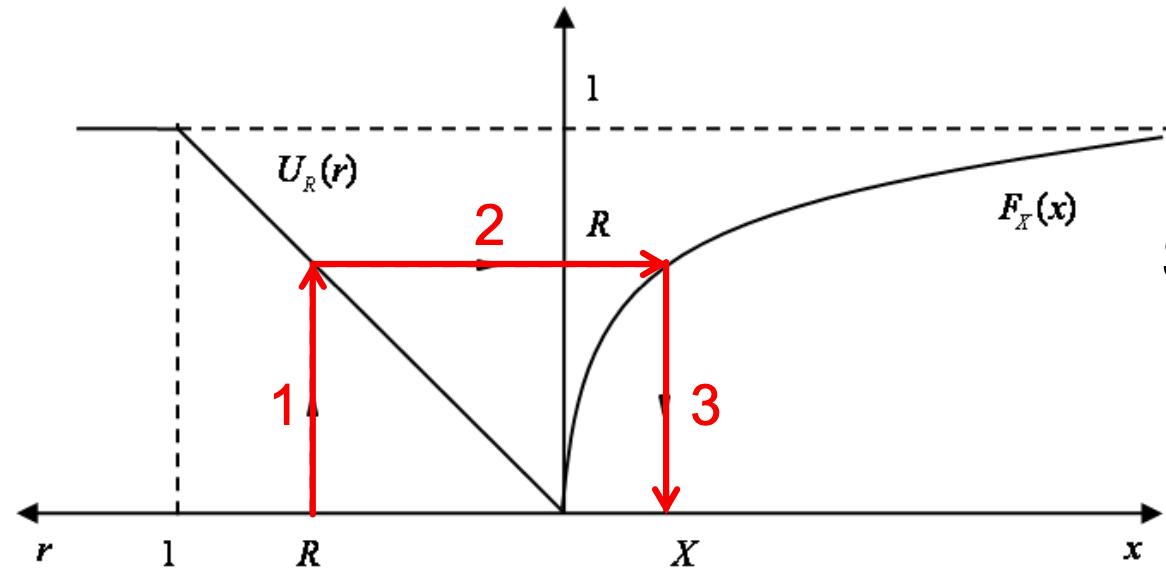
\includegraphics[width=6cm]{Images/Inverse-Transform.png}
\end{center}

For example, we used minimal cut sets in the past to do rare event approximations. With Monte Carlo, we would have to identify states and then do inverse transforms to find the operating states. The arrival state for all arcs in the network are then calculated.The simulation is done for $N$ trials. The estimation of the failure probability is done by dividing the count of failed network states by the number of samples.

\subsubsection*{Sampling from discrete distributions (non-analytical)}

\begin{itemize}
    \item This is the same concept as for the analytical way
    \item However, now we only have dicrete distributions 
    \item This means, that samples $R$ can only achieve a discrete number of outcomes ($X$)
\end{itemize}

\begin{center}
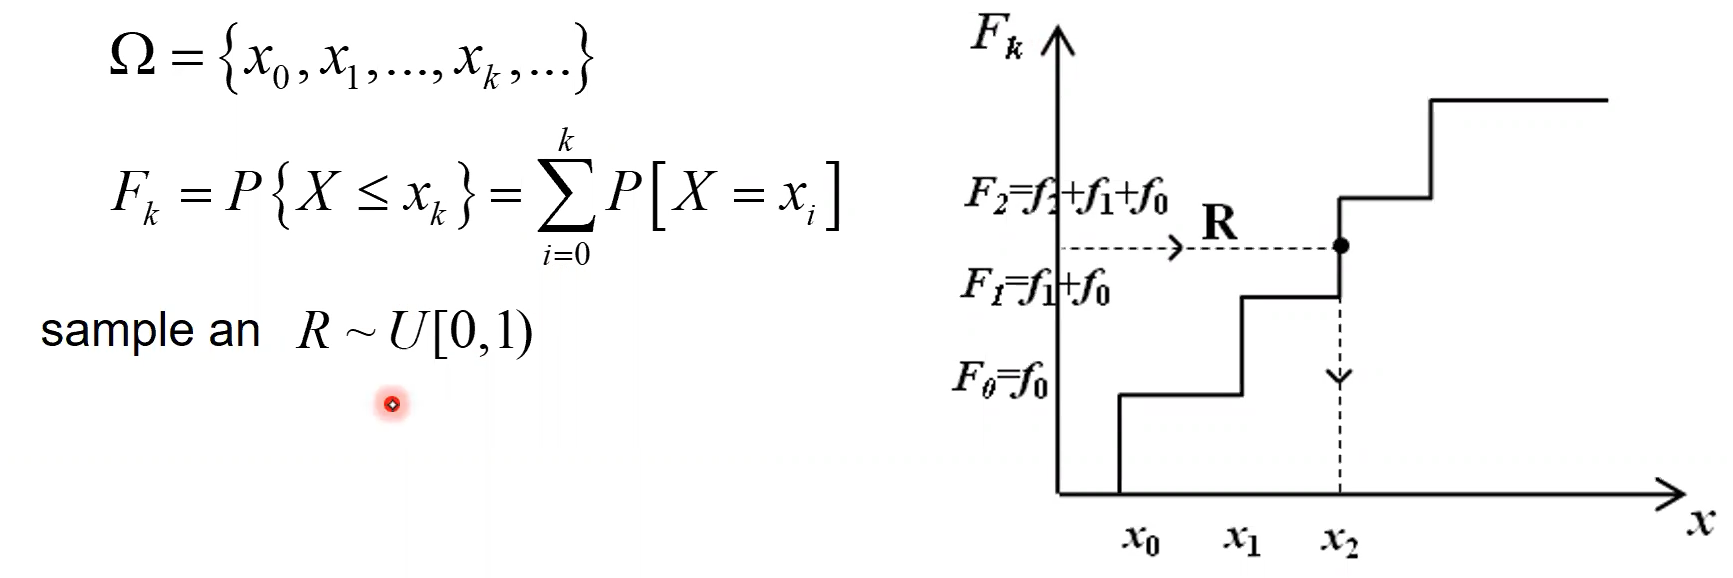
\includegraphics[width=7cm]{Images/Sampling_Discrete.png}
\end{center}


\textbf{Simulation of System Transport}

\begin{itemize}
\item Plant = system of $N_C$ connected components
\item Component = a subsystem of the plant
\item State of the plant at time $t$ = the set/vector of the states in which the $N_C$ components are at t. The plant may be labeled by a scalar which enumerates 
\item Plant transition = When any of the components performs a state transition we say that the plant has performed a transition. The time $t_n$ and state $k_n$ are defined at the $n$-th transition. 
\end{itemize} 


\subsubsection*{Failure Probabilty Estimation: Sampling from discrete distribution}

In class, an example with a network is shown. The rare event approximation is made, as well as the Monte Carlo simulations. With the number of simulations of Monte Carlo, the estimate over a certain number of time will achieve a closer result with a smaller confidence interval. In order to achieve a certain confidence interval, a number of simulations have to be done with a certain number of samples. \newline

\subsubsection*{Stochastic Transitions: Governing probabilities}

\begin{itemize}
    \item $T(t | t'; k') dt = $ conditional probability of a transition at $t \in dt$, given that the previous transition as occured in time step $t'$ and that the state previuosly entered was $k'$
    \item $C(k | k'; t) = $ conditional probability of the plant entering state $k$ from previous time step t. Both probabilities form the "Transport Kernel" $K$ 
\end{itemize}

\begin{equation}
    K(t;k | t';k')dt = T(t|t';k') dt C(k| k';t)
\end{equation}

The ingoing transition density or PDF of a system stransition at $t$, resulting in the entrance in state k. The goal is to to get this PDF (global information) $\psi(t;k)$ 

\begin{center}
    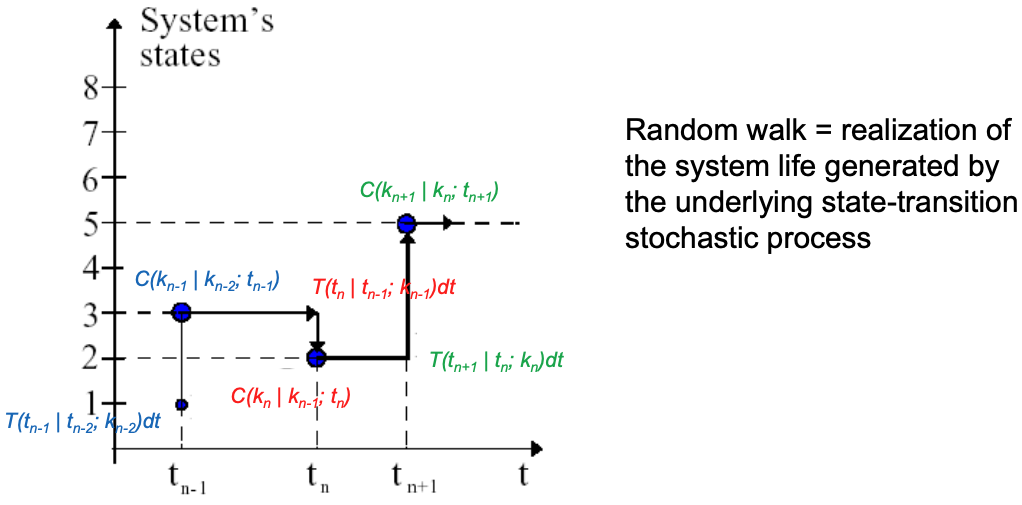
\includegraphics[width=8cm]{Images/RandomWalk.png}
\end{center}

The plant life as an example via random walk = realisation of the system life generated by the underlying state-transition stochastic process. What is required previously? The system state at a previous state. In order to find the new state at the same time, $C$ is sampeled, from which at a later time step $T$ is invoked given the state is known from the previous time step, and so on and so forth. \newline

Random Walk = realization of the system life generated by the underlying state-transition stochastic process \newline

\textbf{System Reliability Estimation}

Counters for Unreliability are defined. We want to compute reliability. As soon as $\tau$ is reached, a failed state has been arrived to. The system could be repaired, and from time horizon $\tau$ until mission time (end of mission) $T_M$ is the relevant horizon. $C^R(t)$ is a counter for unreliability (one monte carlo test). If a failed test is been reached, all timesteps after are adding one towards the monte carlo test. This can be explained similar to a matrix with all time steps from $0$ to $T_M$ width and a height of $M$ Monte Carlo experiments. In the end, the $C$ which is updated with an additional $1$ will be divided into the different number of $M$   


\subsubsection*{Availability and Reliability Estimation}

The availability is estimated through the metric $U(t_j)$, which is the unavailability of the system, whereas the function $C^A(t_j)$ is a counter which only increases as long as the system is in a in failed state which however can be again repaired ($X(t_j) =2$), compared to a failed state where the system cannot be recoverd and hence 

\begin{equation}
    U(t_j) = \frac{c^A(t_j)}{M} = P(X(t_j) = 2)
\end{equation} 

The unreliability counter is added after the first time, the failed state is reached (the system cannot be recovered anymore). The unavailability counter is added until the system is available again.

\subsubsection*{Sample from exponential distribution}

Probability Density Function:

\begin{align}
    f_T(t) &= \lambda e^{-\lambda t}, ~t \geq 0 \\
    &= 0, ~t < 0
\end{align}

Cumulative Distribution Function:

\begin{align}
 F_T(t) &= 1-e^{-\lambda t}, ~t \geq 0 \\
 &= 0, ~t<0
\end{align}

Expected value and variance:

\begin{align}
    E[T] &= \frac{1}{\lambda} \\
    Var[T] &= \frac{1}{\lambda^2}
\end{align}


\section*{Simulation for reliability/availability analysis of a sub-system}

\subsubsection*{Indirect Monte Carlo: Example}

Components' times of transition between states are exponentially distributed, this means that $\lambda_{j_i \rightarrow m_1}^i$ is the rate of transition of component $i$ going from its state $j_i$ to the state $m_i$. On a component level, this means that the transition rate matrix (same as in continuous time Markov) is defined and that the time of transition can be sampled through the summation out of all transitions $\lambda$ from the nominal state for each component, giving a proxi

\begin{equation}
    t_1 = t_0 - \frac{1}{\lambda^{(1,1,1)}} ln(1-R_t), R_t \in [0,1)
\end{equation}

\begin{equation}
    \lambda^{(1,1,1)} = \lambda_1^A+\lambda_1^B+\lambda_1^C
\end{equation}

Assuming that the transition time $t_1$ is smaller than the mission time $T_M$ (otherwise successive trial necessary), it needs to be determined which transition probabilities of each component is:

\begin{equation}
    \frac{\lambda_1^A}{\lambda^{(1,1,1)}}, \frac{\lambda_1^B}{\lambda^{(1,1,1)}}, \frac{\lambda_1^C}{\lambda^{(1,1,1)}}
\end{equation}

The inverse transform method yields a component which undergoes a transition, for example $B$. Hence, giveven that at $t_1$ the component has undergone a transition, the discrete probabilities give mutually exclusive and exhaustive arrival states (since for example only $1$ and $3$ can be reached) from the inverse transform method.

The result of the first transition can be found, and hence the update transition rate could look as follows:

\begin{equation}
    \lambda^{(1,3,1)} = \lambda_1^A + \lambda_3^B + \lambda_1^C
\end{equation}

Finally, the next transition will be calculated as follows:

\begin{equation}
    t_2 = t_1 - \frac{1}{\lambda^{(1,3,1)}} ln(1-R_t)
\end{equation}

The trial simulation proceeds through various transitions from one system configuration to another up to the mission time $T_M$. When the system enters a failed configuration (when C fails) or the minimal cut set, then tallies are appropriately collected for the unreliability (until the end) and instantaneouos unavailability estimates (discrete times $t_j \in [0,T_M)$

In the end, after performng a number of trials $M$, the estimates for unavailability can and unreliabilty can be computed by simply dividing by $M$ the accumulated contents of $C^R(t_j)$ and $C_A(t_j)$

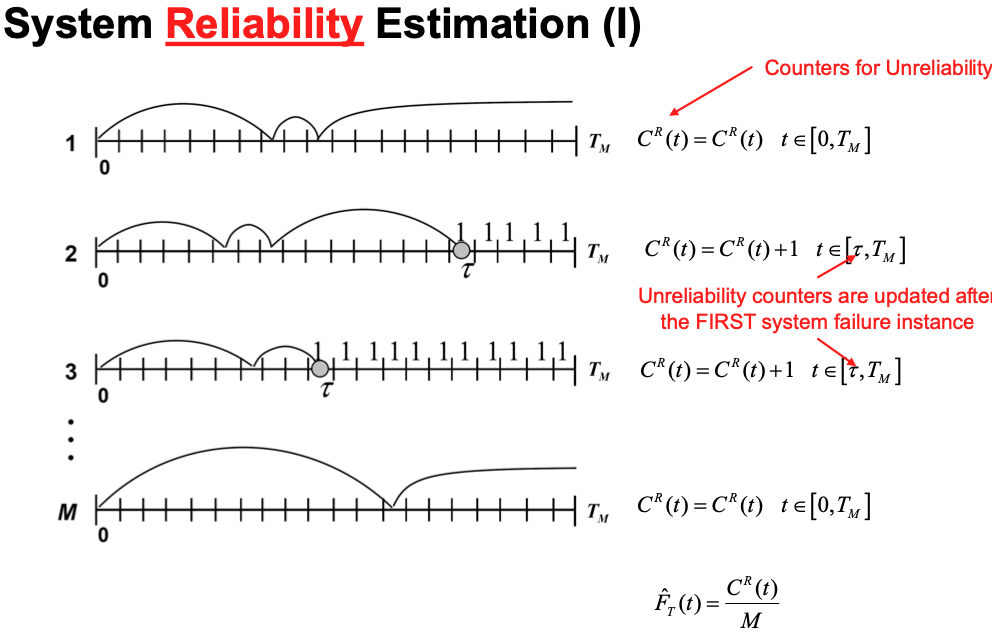
\includegraphics[width=8cm]{Images/Reliability Estimation.png}

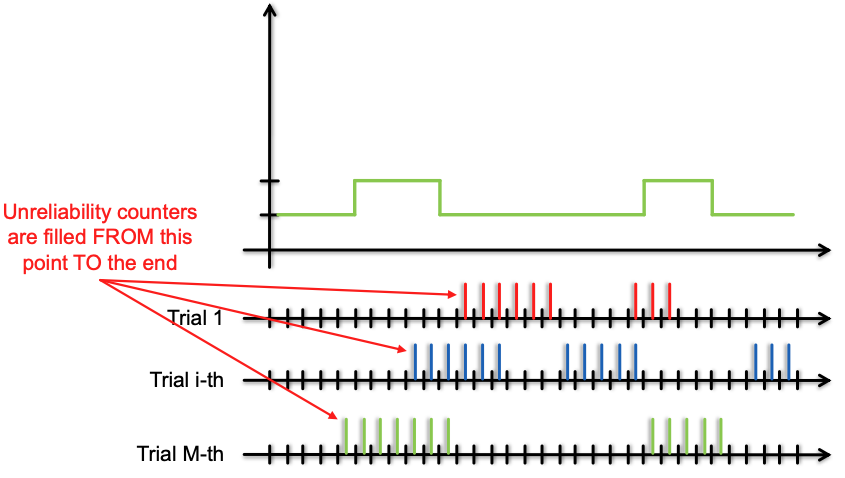
\includegraphics[width=8cm]{Images/Unavailability Estimation.png}

\subsubsection*{Direct Monte Carlo: Example}

For direct Monte Carlo methods, from starting time $t=0$ the system in nominal configuration will be used and all transition times are sampled (not step by step):

\begin{equation}
    t_{1\rightarrow m_i}^{i} = t_0 - \frac{1}{\lambda_{1\rightarrow m_i}^i} ln(1-R_{t,1\rightarrow m_i}^i), R_{t, 1\rightarrow m_i}^i \sim U[0,1)
\end{equation}

\subsubsection*{Sampling the Time and the Type of Transition}

For each and every component, the mission times including time to transition can be estimated. The shortest transition time will then be defined as the new transition time.

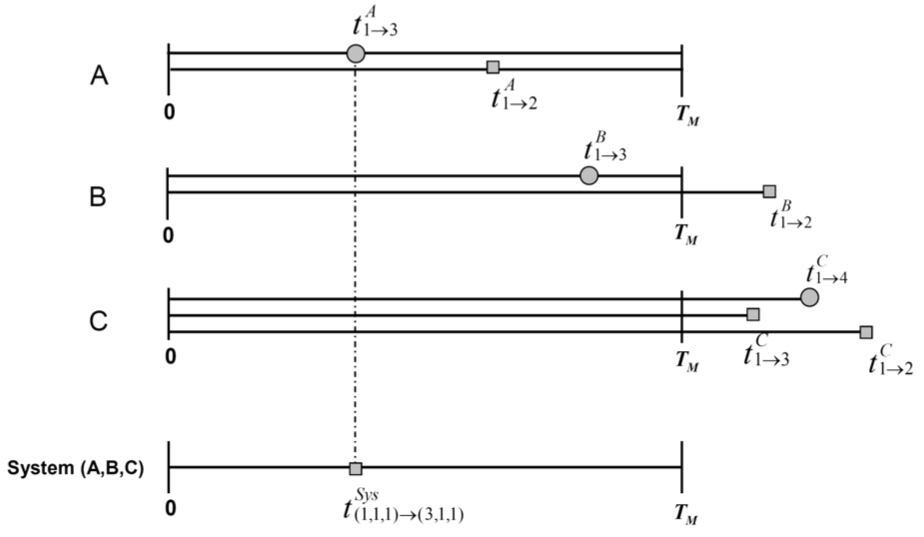
\includegraphics[width=8cm]{Images/TimeAndTypeOfTransition.png}

The simulation proceeds to the successive times in the list, in correspondence of which a system transition occurs. After each transition the timeline is updated with the times of the transition that the component has undergone the last transition can do from its new state. The unreliability and unavailability estimates are computed each time the system enters a failed configuration.

\subsection*{Offshore Installation: Example of indirect Simulation for a multi-state system}

\subsubsection*{Structure of Monte Carlo Code}

\begin{itemize}
    \item Set the number of MC repetitions, the mission time
    \item Set the input for each component state and transition rate across states
    \item Set the counter structure (availability and reliability)
    \item For loop for MC trials (repetitions, histories)
    \item Initialization of system state vector, reset time)
    \item While $t < $ Mission time 
    \begin{itemize}
        \item Mapping the state of the components to the system state
        \item Take the step to the random walk $\rightarrow$ Compute the transition rate out of initial state
        \item Sample from the $T$ and $C$ the transition time and the arrival state
        \item Update the counters
    \end{itemize}
\end{itemize}


The analytical approach of a Markov model becomes impractical, as soon as the system becomes highly complex. This means, that if for example the number of components, their states (hence many plant states) and for example repair teams (which can modify plant states) can yield a inhomogeneous Markov chain. Therefore, Monte Carlo is used whereas system faults will be grouped. Different minimum cut sets are defined. The transport kernel is defined as always, through sampling from the exponential distribution. 

%% 22. April

\subsection*{Monte Carlo - The theoretical view}

\subsubsection*{Sampling random variables}

\textbf{Sampling in uniform}

\begin{itemize}
    \item cdf: $U_R(r) = P(R \leq r) = r$
    \item pdf: $u_R = 1 = \frac{d U_R}{dr}$
\end{itemize}

\textbf{Pseudo random numbers in uniform}

\begin{itemize}
    \item $x_i = (ax_{i-1} + c)~mod~m$
    \item where $a$, $c \in [0,m-1)$ and $m>>1$ are free parameters 
    \item $r_i = \frac{x_i}{m}$
    \item As a result, the pdf of the analytical function can be well approximated
\end{itemize}

\textbf{Buffon's Needle} is a method which lets us approximate $\pi$. The idea is stemming from the fact that a needle of length $L$ with a size smaller than $D$ spaced lines has a certain probability of intersecting with one line. The needle is randomly oriented by its angle $\phi$ and its center height $y$ which are independent from each other. For a fixed $\phi$, the probabilty is just a function of $y$:

\begin{itemize}
    \item $P(Y \leq L sin\phi) = \frac{L sin\phi}{D}$
\end{itemize}


For a random variable $\phi$, the probability is:

\begin{itemize}
    \item $P = \frac{2L}{\pi D}$
\end{itemize}

The counter is initialised via $N_S = 0$ at the beginning. Since the pdf is $f_Y(y) = \frac{1}{D}$ the reverse transform method will yield: $R = \frac{Y}{D}$ and $Y = R_1 D$, whereas the angle is similarly sampled: $\Phi = R_2 \pi$. If the needle intercepts the line, the $N_S = N_S +1$. In the long term, $P \approx \frac{N_S}{N}$ and hence $\pi$ can be approximated through the given formula. \newline

\textbf{Constant rate exponential distribution}

Assuming we have a markovian state (2 states, good and failed), and a constant hazard rate $\lambda = const.$ The following equations hold true:

\begin{itemize}
    \item $R = 1-e^{-\lambda t}$
    \item inverted: $T = F^{-1} = -\frac{1}{\lambda} ln(1-R)$
\end{itemize}

\textbf{Time-dependent rate Weibull distribution} - if the hazard rate is not constant

\begin{itemize}
    \item $R = 1-e^{-\beta t\alpha}$
    \item inverted: $T = F^{-1} = \left(-\frac{1}{\beta} ln(1-R)\right)^{\frac{1}{\alpha}}$
\end{itemize}

\textbf{Sampling from non-invertible transition time pdf} - if for example the pdf is not analytically invertible (mathematically for example $f_T^{i,j_i \rightarrow m_i}(t) = 0.453 e^{-1.036 t}\sinh \sqrt{2.29 t}$, or if goint to infinite somewhere when $x$ is zero or so). Then, the $t_S$ is sampled via interpolation between two points in the distribution.

\begin{equation}
   t_s = x_1 + \frac{x_2 -x_1 }{F_2 - F_1 } (R_S - F_1)
\end{equation}

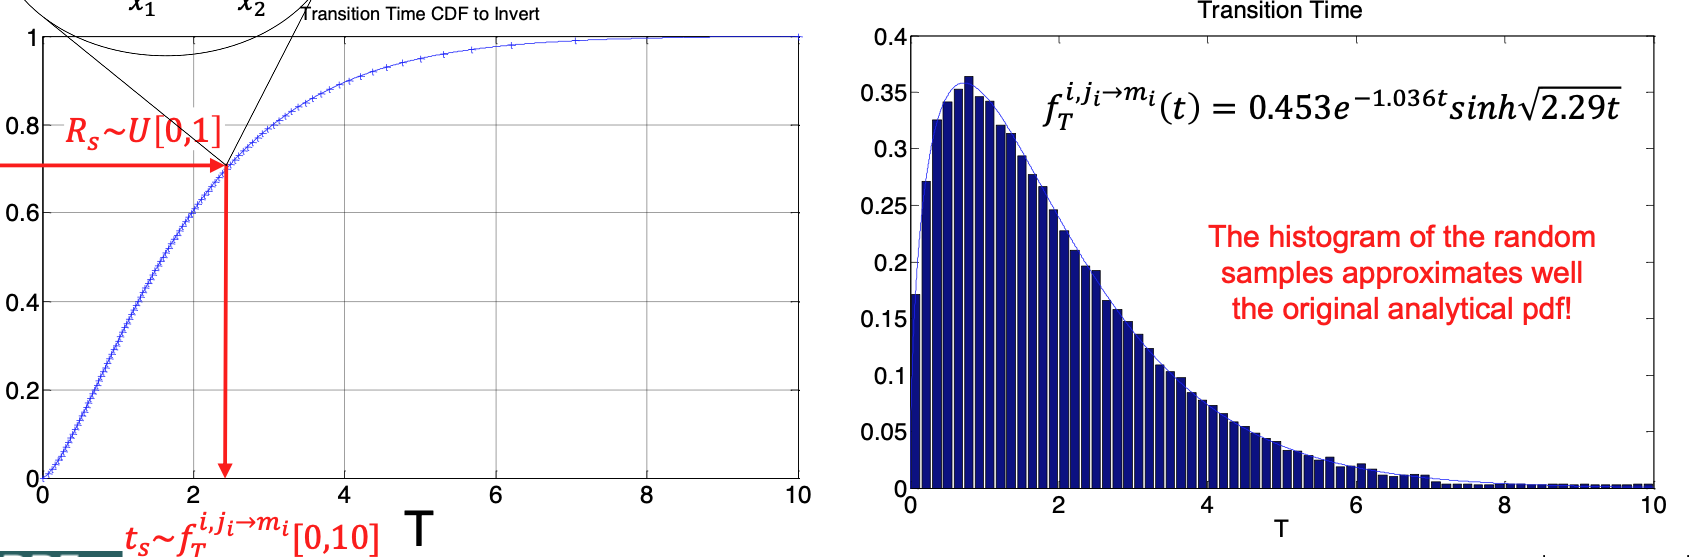
\includegraphics[width=10cm]{Images/SampledInterpolationNonInvertible.png}

The histogram of random samples approximates the function pretty well. \newline

\textbf{Von Neumann Algorithm I (Sampling by Rejection)} \newline

If a pdf is complicated, then normalize the maximal point such that it becomes one and a point $f_X(x)$ is between $0$ and $1$:

\begin{equation}
    h(x) = \frac{f_X(x)}{f_M}
\end{equation} 

Then sample a $x'$ between the beginning and end of the function and calculate its function value $h(x')$, which is called a \emph{tentative value}. Sample a R between 0 and 1 and accept it iff it is smaller than $h(x')$. \newline

\textbf{Von Neumann Algorithm II} \newline


%%29. April


We assume that now we can split up the function $f_X(x)$ into a product of $g_X'(x)$ and $H(x)$, which is possible based on theoretical assumptions. The maximum will be defined as previously, hence $B_H = max(H)$ and therefore $h(x) = \frac{H(x)}{B_H}$, the same procedure is done as shown previously, where if the sample is inbetween the tentative value and 0, we accept the sample. The efficiency of the rejection method is:

\begin{equation}
    \epsilon = P[accepted] = \frac{1}{B_H}
\end{equation}

In the following example, a trick is used to decouple two functions. One trick would be to define $X = R^2$, meaning that the random variable is a square of another one. This eliminates the terms with squareroots in the denominator of a pdf due to the derivative a square root. 

\subsection*{MC Evaluation of Definite Integrals (1D)}

The function which yields an award, such as $G$ can be defined as follows:

\begin{equation}
    G = \int_a^b g(x) f(x) dx 
\end{equation}

assuming $f(x)>0$ and a pdf $\int f dx = 1$, $G$ is equal the \textbf{Expectation Value} $E(g(x))$, meaning the expected outcome of a function $g$ which awards a sampled $x_i$. Considering $N$ trials, the expected win is the average of sampled $g$

\begin{equation}
    G_N = \frac{1}{N} \sum_{i=1}^N g(x_i) = \overline{g}
\end{equation} 

In order to prove why $G_N$ is a good estimator, the \textbf{Expectation and Variance} of $G_N$ can be computed. The expectation value is exactly $G$ and the variance is zero, when using the above definition of $G_N$. With $N \rightarrow \infty$, the variance vanishes to zero. Even though one could always compute the values numerically, those are not always known in practical cases due to the complexity of the problem. \newline

\textbf{Biased case (Importance Sampling)}

If however $f$ and $g$ are such that one is big and the other is small, then for example the variance becomes huge nad hence error of the estimate as well. 

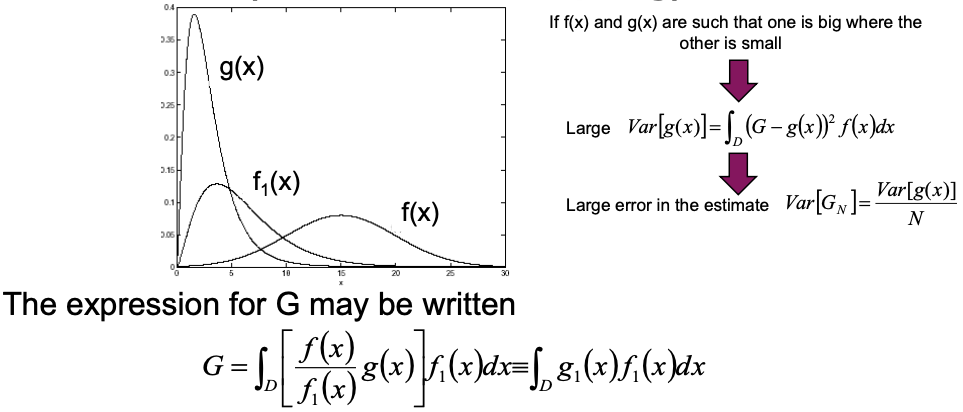
\includegraphics[width=8cm]{Images/BiasedSampling.png}

In order to mitigate the error, the following equation is used:

\begin{equation}
    G =  \int_D \left[ \frac{f(x)}{f_1(x)} g(x)\right] f_1(x) dx = \int_D g_1(x) f_1(x) dx
\end{equation}

The biasing happens by shifting the center towards the other center through scaling and translation. The award is now a function of $g_1$ instead of $g$ and the award is $G_{1N}$. By using the taylor expansion of $g(x)$ (a polynomial) and then through a normalisation procedure, $g$ is ultimately approximated.

\subsubsection*{Simulation of System Transport}

The von Neumann approach of the random walk is motivated by having the system transport kernel, a function of the conditional probability transition and the conditional probability that a system enters a state - whereas a new function $\psi$ is defined as a series of transitions and independent of previous states and time steps. \textbf{The transition density $\psi(t;k)$ is expanded in a series of the partial transition densities $\psi^n(t;k)$} (n-th transition at $t$, entering $k$):

\begin{equation}
    \psi(t,k) = \psi^0(t,k) + \sum_{k'} \int_{t_0}^t \psi(t',k')K(t,k | t',k') dt
\end{equation}

The term in the integral is a convolution term, whereas the transport kernel is convoluted with $\psi$ from the previous time and state. The transition density of the previous time step is however again a transport kernel (see figure) and so this results into a multidimensional convolution for higher order system transport kernel. 

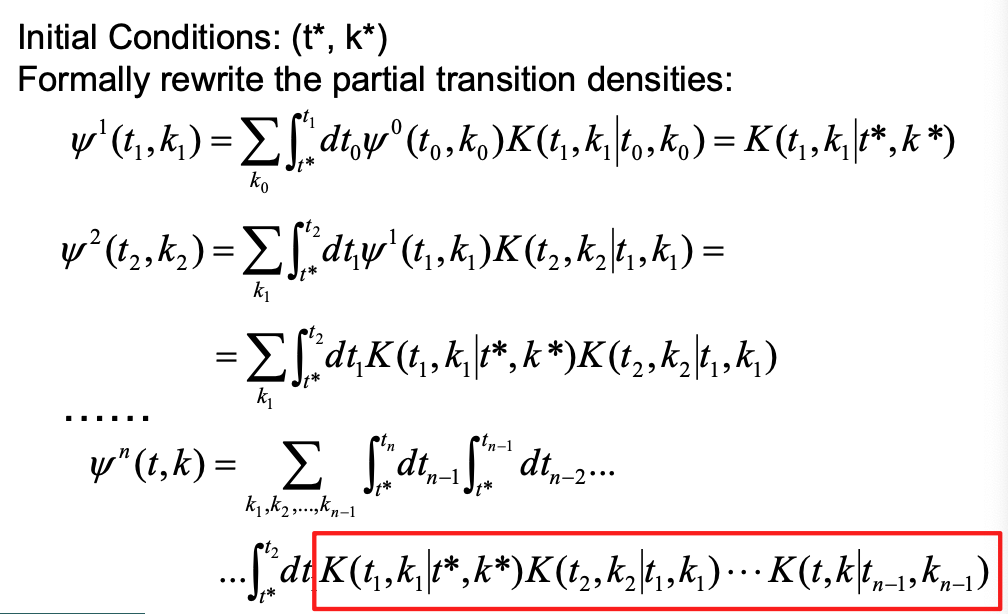
\includegraphics[width=8cm]{Images/TransportEquationSystem.png}
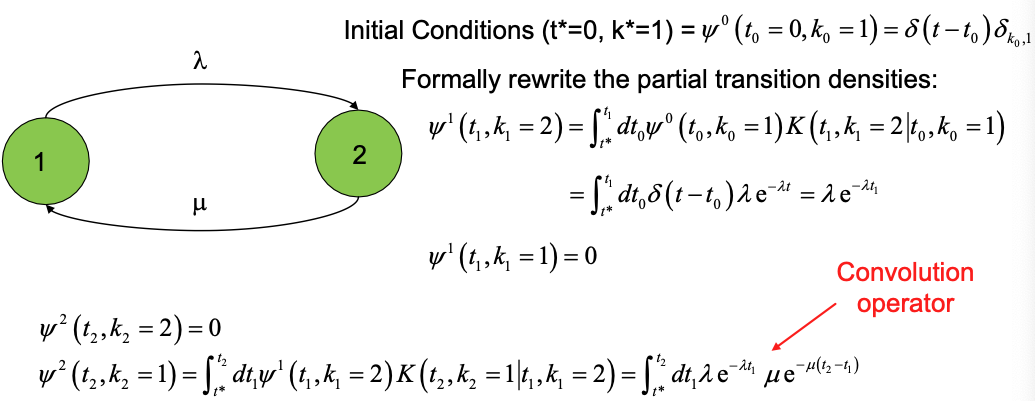
\includegraphics[width=8cm]{Images/TransportEquationExampleConvolution.png}
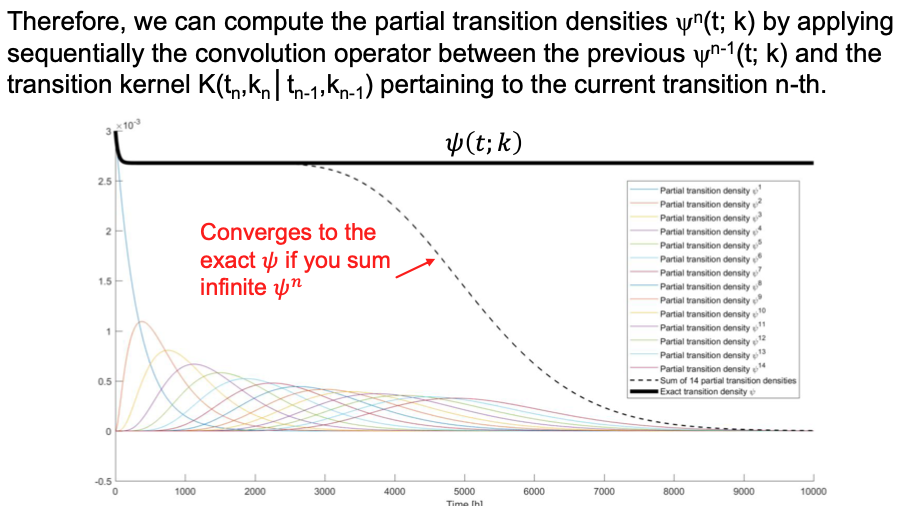
\includegraphics[width=8cm]{Images/ConvergenceOfPsi.png}
\subsubsection*{Simulation for Reliability and Availability Analysis}

%% 20. May lecture

\end{multicols*}
\end{document}

